\chapter{Experimental Evaluation}\label{ch:experimental_evaluation}

This chapter presents results of experiments that were conducted in order to evaluate the use of DRL for robotic grasping with octree-based observations. The created simulation environment is analysed with respect to the feasibility of sim-to-real transfer in order to validate the applicability of all results for use in real-world domain. Furthermore, various configurations and ablations are studied to provide comparative investigation of different approaches and their advantages for learning robotic manipulation with DRL.


\section{Experimental Setup}

All experiments utilise the simulation environment for the training of all RL agents. Generalisation to novel objects is evaluated for all agents in the same simulation but on a testing dataset, where one of the trained agents is in addition evaluated also on a real robot.


\subsection{Simulation}

Unless otherwise stated, the training in simulation is identical to the setup described in \autoref{sec:impl_simulation_environment} with full-scale domain randomisation. UR5 robot with RG2 gripper is utilised as the primary robot for all experiments because it is the robot that is also tested in real-world domain. However, one of the agents is trained using the Panda robot. Panda is also used to evaluate possible generalisation to new robots with an agent trained on UR5, and vice versa. The same random seed is used to train all agents.

When evaluating the trained agents, testing datasets for both object models and PBR textures are used. The environment is configured to present the agent with the full task, i.e.~largest possible workspace and maximum number of objects. Each episode can last at most~100 time steps and agent succeeds only if an object is lifted~12.5~cm above the ground. The random seed is changed for all evaluated agents to a new common value that is different from a seed used during training. In order to encourage reproducibility, this simulation setup is available as a pre-built Docker image\footnote{\href{https://hub.docker.com/r/andrejorsula/drl_grasping}{https://hub.docker.com/r/andrejorsula/drl\_grasping}}.


\subsection{Real}

Real world setup shown in \autoref{fig:real_setup} is used to evaluate sim-to-real transfer. This setup consists of a UR5 robot with RG2 gripper and Intel RealSense D435 RGB-D camera\footnote{\href{https://intelrealsense.com/depth-camera-d435}{https://intelrealsense.com/depth-camera-d435}} that is mounted on a tripod in front of the robot. Pose of the camera with respect to the robot is calibrated with a procedure described in \hyperref[app:calibration]{appendix~\ref*{app:calibration}}. Similarly, \hyperref[app:camera_configuration_and_postprocessing]{appendix~\ref*{app:camera_configuration_and_postprocessing}} presents the configuration and post-processing of the camera output.

\begin{figure}[ht]
    \centering
    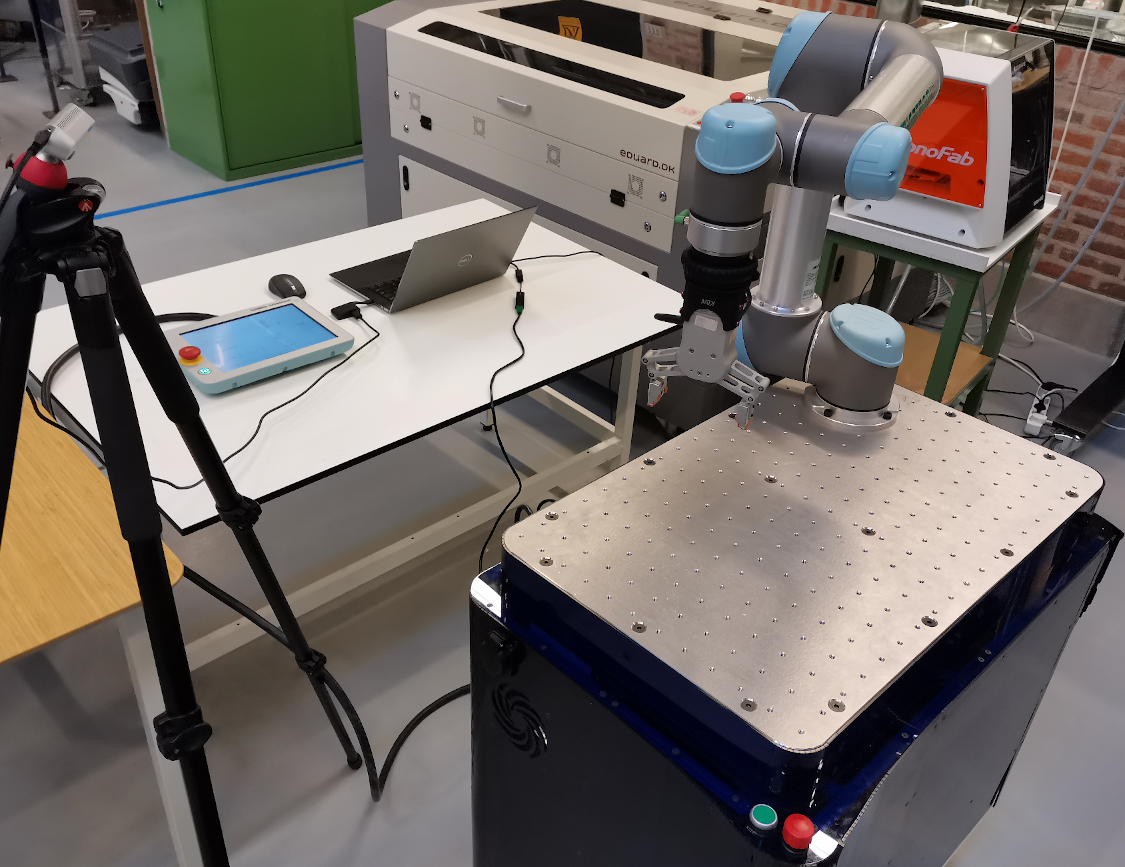
\includegraphics[width=0.75\textwidth]{experimental_evaluation/real_setup.png}
    \caption{UR5 robot with RG2 gripper and RealSense D435 camera in a setup that is used to evaluate sim-to-real transfer.}
    \label{fig:real_setup}
\end{figure}

\autoref{fig:real_objects} shows~18 different objects that were used in real world during the testing. Mostly compliant objects were selected in order to reduce the risk of damage to the gripper due to the unpredictability of end-to-end RL policy trained in a different domain. The same workspace volume and number of objects are used as in the simulation. Similarly, the goal of the agent is to lift an object within~100 time steps.

\begin{figure}[ht]
    \centering
    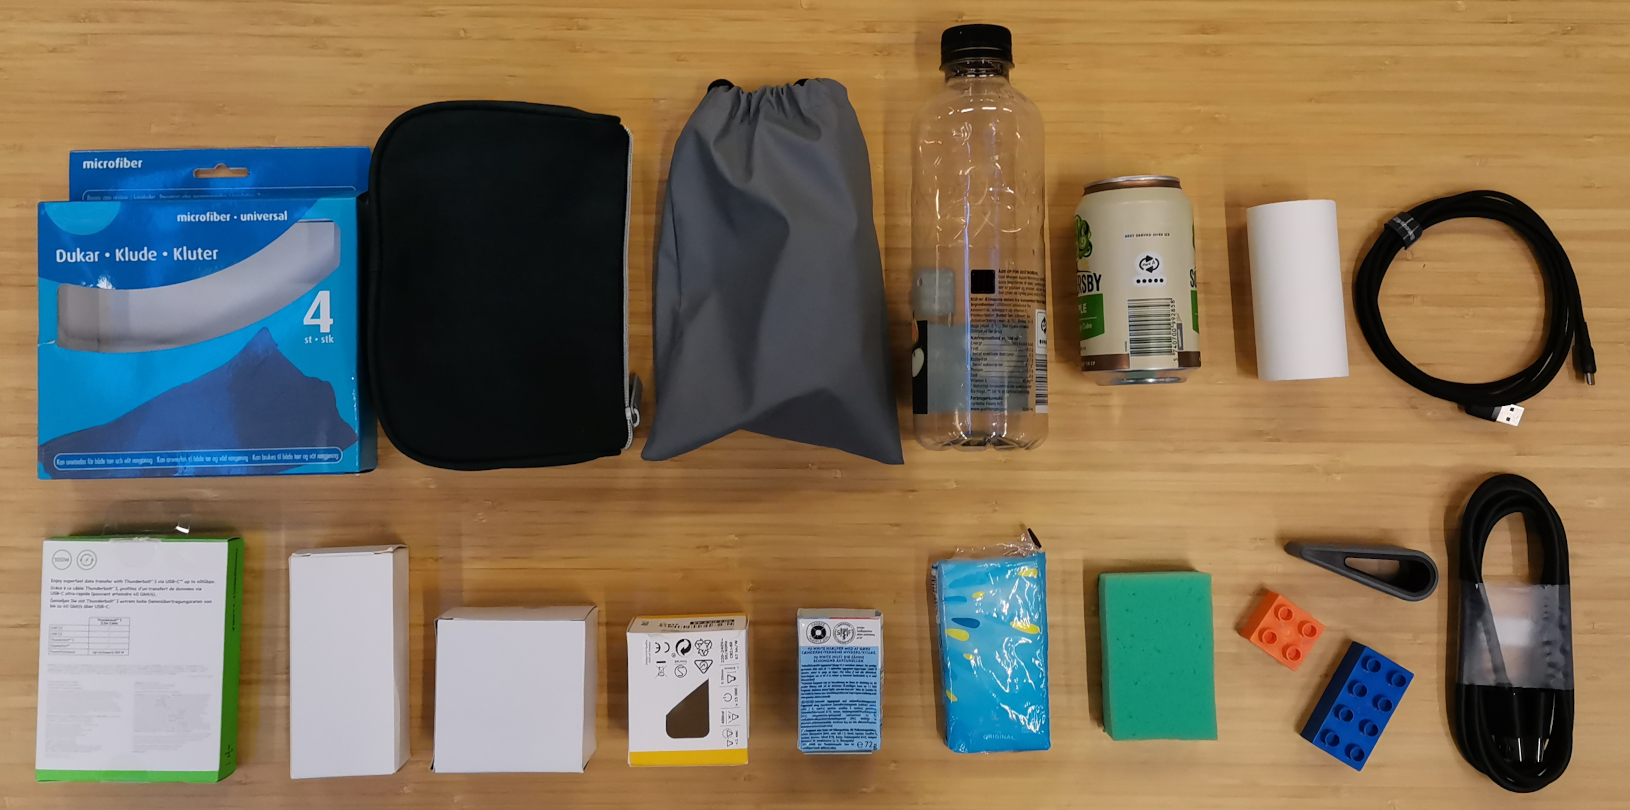
\includegraphics[width=0.75\textwidth]{experimental_evaluation/real_objects.png}
    \caption{A set of 18 objects used during the sim-to-real evaluation.}
    \label{fig:real_objects}
\end{figure}


\section{Results}

\subsection{Comparison of Actor-Critic Algorithms}

\subsection{Comparison of 2D/2.5D/3D Feature Extraction}

params:
    octree - 226384
    rgb -
    rgbd - 227822 (or 229766)


\subsection{Invariance to Robot}

\subsection{Invariance to Camera Pose}

\subsection{Sim-to-Real Transfer}

41/60 success
- 68\%


\section{Ablation Studies}

\subsection{Curriculum}

\subsection{Demonstrations}

\subsection{Colour Features}

\subsection{Proprioceptive Observations}

\subsection{Sharing of Feature Extractor between Actor and Critics}

\subsection{Separate Feature Extractors for Stacked Observations}

